\documentclass{article}

\usepackage[utf8]{inputenc}

\usepackage{siunitx}		% si units
\usepackage{graphicx}	% images
\usepackage{amsmath, amssymb, amsthm}
\usepackage{textcomp}	% degree symbol

\usepackage{booktabs}	% better tables

\usepackage{listings}		% code listings with highlighting
\usepackage{courier}		% change listings to courier font


\lstset{basicstyle=\footnotesize\ttfamily,breaklines=true}
\lstset{framextopmargin=50pt,frame=bottomline}
\lstset{showstringspaces=false}

\graphicspath{ {images/} }


\title{Structure and oxygen affinity of myoglobin: an MD study}
\author{Jason \textsc{Weinzierl} \\
\textit{Department of Physics and Astronomy,} \\
\textit{University of Missouri, Columbia, Missouri 65211-7010, USA}}
\date{(\today)}

\begin{document}

\maketitle

\begin{figure}[h]
	\centering
	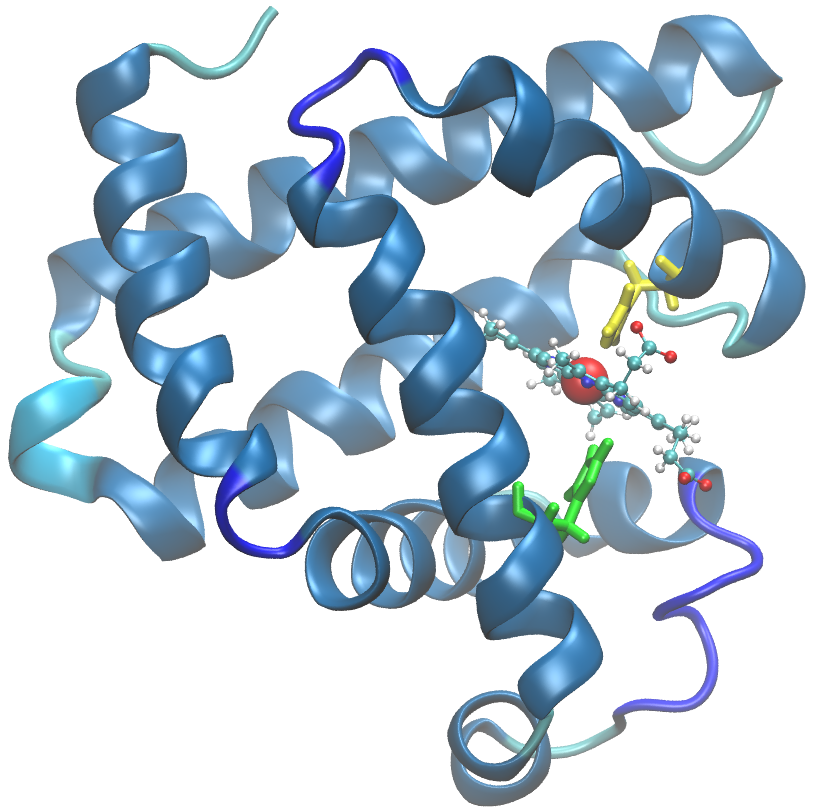
\includegraphics{myoglobin.png}
\end{figure}

\begin{abstract}
Using molecular dynamics simulations and visualization software, we investigate the small protein \textbf{myoglobin}.  We find that the protein's structure is generally conserved across species.  We also demonstrate with MD simulations that oxygen enters myoglobin through cavities which open and close with thermal fluctuations.  Finally, we show that myoglobin resists fatal binding with carbon monoxide by restricting the binding angle to the heme group.
\end{abstract}

\section{Introduction}

Myoglobin is a globular protein found in the muscle of vertebrates.  It binds to oxygen and is similar to hemoglobin, the oxygen-carrier found in blood.  Myoglobin acts a pigment in muscle tissue, coloring it red.  The function of this 154-residue protein is thought to be oxygen storage.  At the heart of myoglobin is a heme group with an atom of iron in the center (Figure~\ref{fig:heme}).

In this project, we will study the general structure of myoglobin and its conservation across species, as well as investigating how it fulfills its role in reversibly binding with oxygen.  We will simulate the protein to look at how oxygen gets past the protective alpha-helices to bind with the heme.  We will also look at how myoglobin resists binding with CO, which is irreversible and catastrophic to the molecule.

\begin{figure}
	\centering
	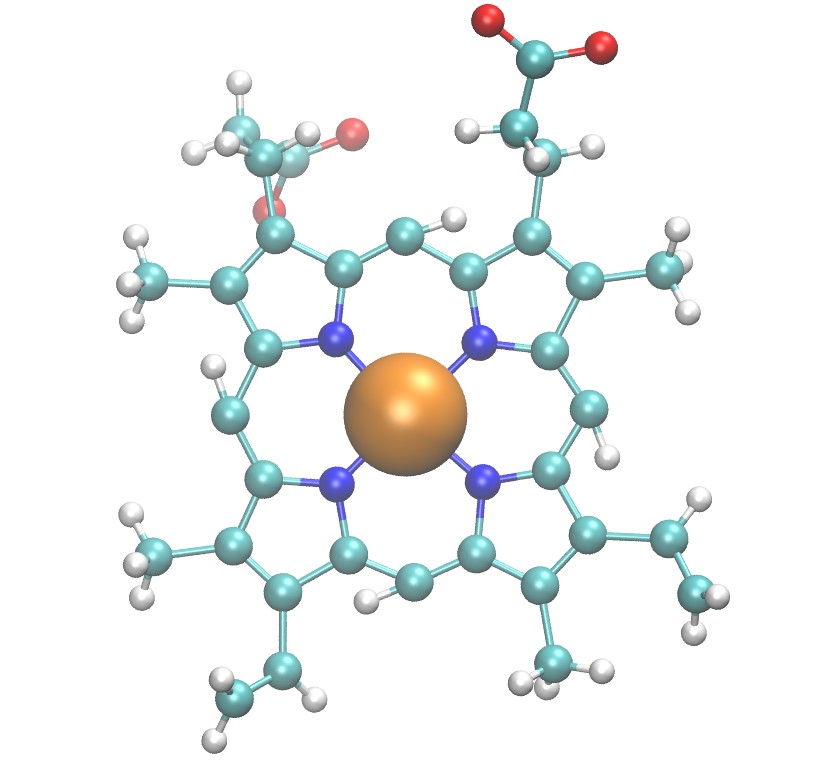
\includegraphics[width=0.5\textwidth]{heme.png}
	\caption{The heme group, featuring the orange iron atom at the center, supported by four N atoms.}
	\label{fig:heme}
\end{figure}



\section{Methods}

\subsection{Visualizing structure}

We first will use VMD to display the eight alpha-helices of the protein, the heme group with an iron in the center, the \textbf{proximal histidine} anchoring the heme, and the distal histidine which will come into play when investigating binding angle.

For presenting the ubiquity of myoglobin, we obtain the following crystal structure files from the protein databank:

\begin{itemize}
	\item \lstinline|aplysia-1MBA.pdb|
	\item \lstinline|horse-1WLA.pdb|
	\item \lstinline|seal-1MBS.psb|
	\item \lstinline|tuna-1MYT.pdb|
	\item \lstinline|turtle-1LHS.pdb|
	\item \lstinline|whale-1MBC.pdb|
\end{itemize}

We use a TCL script (Appendix~\ref{lst:loadalign}) to load these structures and color them on input.  However, the loaded proteins are not aligned (Figure~\ref{fig:loadalign}).

\begin{figure}
	\centering
	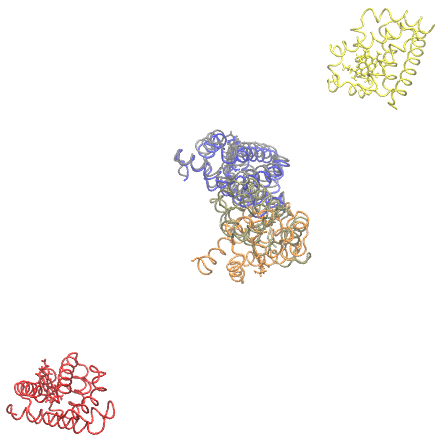
\includegraphics[width=0.5\textwidth]{loadalign.png}
	\caption{Default view on initial import of proteins.  This is unacceptable for visualization.}
	\label{fig:loadalign}
\end{figure}

So we will use a VMD Extension called MultiSeq to align the proteins (Extension > Analysis > MultiSeq).  We will point out, based on the understood function of myoglobin, which residue sequences are most conserved.  We expect from the literature that the \textit{Aplysia limacina} myoglobin will be most different from the others \cite{tutorial}, and will point out the major differences.

\subsection{Demonstrating oxygen access}

Myoglobin is tightly packed with side groups to protect the heme from oxidizing or binding with other unwanted molecules.  This also shields the heme from oxygen.  Yet, we know that oxygen must reach the heme group somehow.  From a static picture, we will show that there are no `oxygen channels'.  But we should find, over time, that cavities arise due to thermal fluctuations of the residues.  The probabilistic motion spreads cavities throughout and eventually allows O2 to reach the heme.  Note: I stated incorrectly in my presentation that this happens on the femtosecond timescale, when it in fact happens in a \emph{much} longer process, from nanoseconds to microseconds \cite{tutorial}.

In order to demonstrate this, we will first use NAMD to simulate a short demonstration, displaying the random cavity openings.  Then we will attempt to run a much longer simulation and show a possible oxygen pathway to the heme.

\subsection{Building heme simulations}

Finally, we want to show how myoglobin resists binding irreversibly to carbon monoxide.  On the oxygen-binding side of the heme, the \textbf{distal histidine} is believed to enforce a shallow binding angle.  We define this \textbf{binding angle} as the Fe--O--O or Fe--C--O angles for oxygen or carbon monoxide molecules respectively.

% TODO: energetic cost associated with enforcing a shallow binding angle

% TODO: slug binding site might have different function

So if a shallow binding angle is enforced in myoglobin, then we will show the desired binding angles of CO and O$_2$ to the heme in a water box.  CO should remain nearly straight, while oxygen should have a more shallow angle with a larger RMSD.  These simulations will be run for \SI{500}{\pico\second}, and we will plot the angles over time, demonstrating averages and RMSD fluctuation in the angle.

\section{Results and Discussion}

\subsection{Structure and conservation across species}

Figure~\ref{fig:alpha_helices} shows the strong helix structure of myoglobin, and Figure~\ref{fig:histidines} shows the two histidines and bound oxygen on the heme.  The unbounded heme group was shown previously in Figure~\ref{fig:heme}.

\begin{figure}
	\centering
	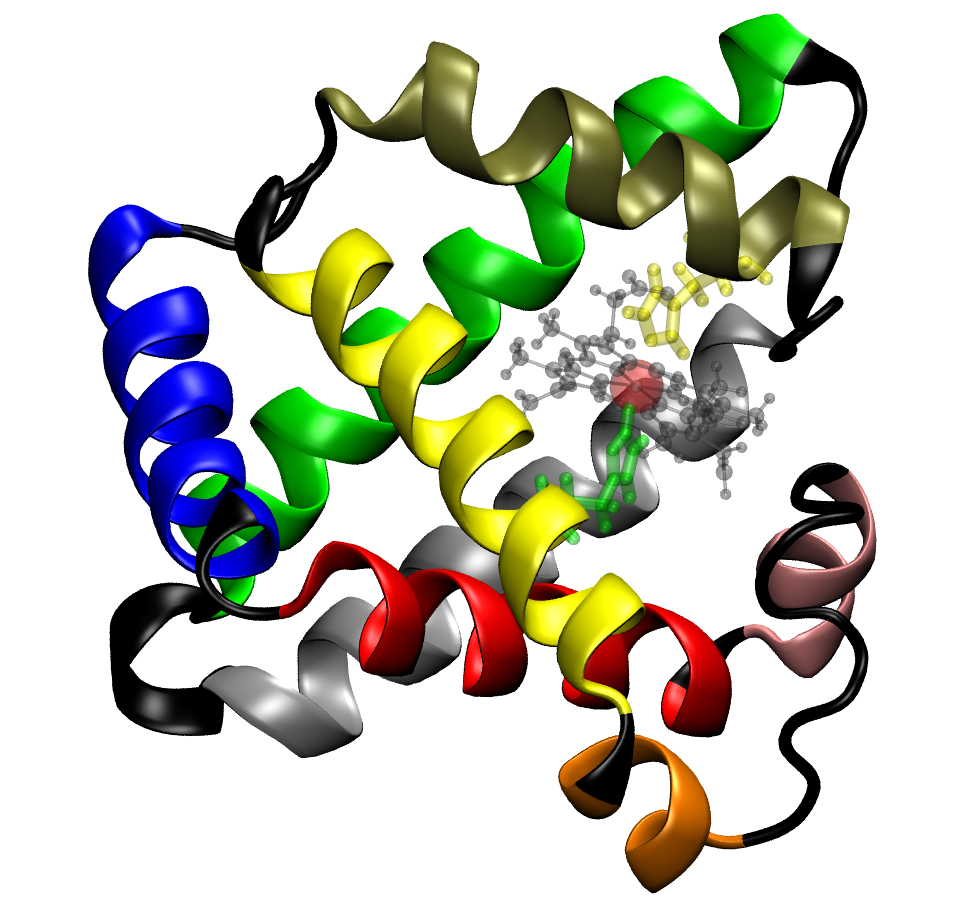
\includegraphics[width=0.5\textwidth]{alpha_helices.png}
	\caption{The eight alpha helices of whale myoglobin.  Alpha helix 1 (residues 4 to 18) is colored blue, helix 2 (21 to 35) is red, helix 3 (37 to 42) is pink, helix 4 (52 to 57) is orange, helix 5 (59 to 77) is yellow, helix 6 (82 to 96) is bronze, helix 7 (101 to 119) is silver, and helix 8 (125 to 149) is green.  The rest of the secondary structure is in black and the heme/histidines core is transparent.}
	\label{fig:alpha_helices}
\end{figure}

\begin{figure}
	\centering
	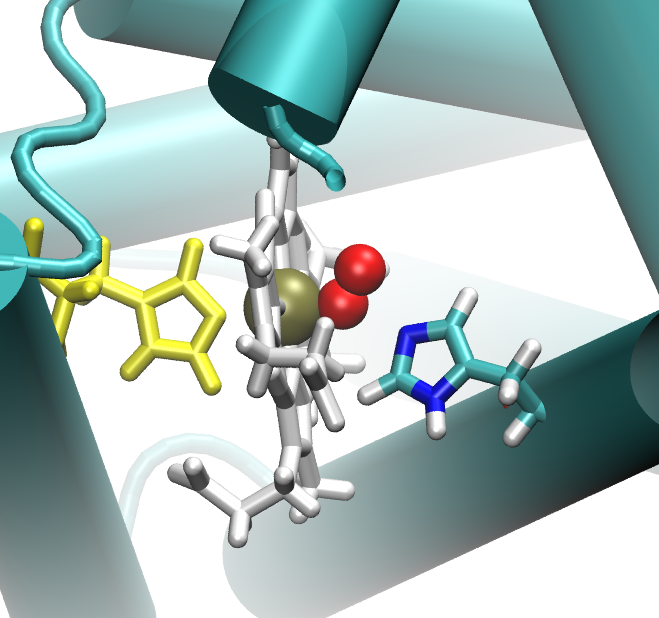
\includegraphics[width=0.5\textwidth]{histidines.png}
	\caption{The heme, colored white with a bronze FE, bound to red oxygen.  The heme is anchored to the proximal histidine, in yellow.  The distal histidine, colored by atom name, enforces a shallow binding angle to the iron center.}
	\label{fig:histidines}
\end{figure}

Now we look at myoglobin of six different species: \textit{Aplysia limacina} (mottled sea hare), \textit{Equus caballus} (horse), \textit{Phoca vitulina} (seal), \textit{Thunnus albacares} (yellowfin tuna), \textit{Caretta caretta} (sea turtle), and \textit{Physeter macrocephalus} (sperm whale).  Figure~\ref{fig:species} shows the six myoglobins overlayed.

\begin{figure}
%	\centering
%	\includegraphics[width=0.5\textwidth]{species.png}
%	\caption{}
%	\label{fig:species}
\end{figure}

TODO: fix coloring of species to make the differences more pronounced in the VMD image.

\subsection{Oxygen pathways}
This is a long simulation, still working on configuration file.

TODO: fix current representation to highlight oxygen in cavities, then simulate the longer pathway simulation

\subsection{Binding angles of O$_2$ and CO}
TODO: use water box scripts from class, obtain pdb files of heme bound to CO or O2, simulate.


\section{Conclusion}

We've displayed the structures of myoglobin across species, simulated oxygen's entry, and showed how it resists CO binding.

\appendix

\section{loadalign.tcl}
\label{lst:loadalign}

\begin{lstlisting}
mol delete all
foreach species {whale-1MBC aplysia-1MBA horse-1WLA seal-1MBS tuna-1MYT turtle-1LHS} {
  mol new $species.psf waitfor all
  mol addfile $species.pdb waitfor all
  mol modstyle 0 top Tube 0.300000 6.000000
  mol modcolor 0 top Molecule
  mol addrep top
  mol modselect 1 top resname HEME
  mol modstyle 1 top Licorice 0.300000 8.000000 6.000000
  mol modcolor 1 top Molecule
}
\end{lstlisting}

\begin{thebibliography}{9}
\bibitem{tutorial}
	Anton Arkhipov, Rosemary Braun, and Ying Yin,
	\textit{Case Study: Myoglobin},
	University of Illinois at Urbana-Champaign, Illinois,
	21 February 2008.
	
\bibitem{vmd}
	Humphrey, W., Dalke, A. and Schulten, K., `VMD - Visual
	Molecular Dynamics', J. Molec. Graphics 1996, 14.1, 33-38.

\bibitem{secondary}
	Frishman,D \& Argos,P. (1995) Knowledge-based secondary structure
	assignment. Proteins: structure, function and genetics, 23, 566-579.

\end{thebibliography}

\vspace{\fill}

\centering{Prepared with \LaTeX.}


\end{document}